

\documentclass[colorlinks=true,pdfstartview=FitV,linkcolor=blue,
            citecolor=red,urlcolor=magenta]{ligodoc}

\usepackage{graphicx}
\usepackage{amssymb}
\usepackage{amsmath}
\usepackage{longtable}
\usepackage{rotating}
\usepackage[usenames,dvipsnames]{color}
\usepackage{fancyhdr}
\usepackage{subfigure}
\usepackage{hyperref}
\ligodccnumber{T}{11}{XXXXX}{}{vX}% \ligodistribution{AIC, ISC}

\graphicspath{{images/}}
\title{Quantization Noise in Digital Control Systems}

\author{Ayush Pandey}


\begin{document}


 \section{Introduction}
    \subsection{General Technical Area}
The project would see its application in the Advanced Laser Interferometer Gravitational Wave Observatory (aLIGO) which is an upgrade over the original LIGO \cite{LIGO} setup. The LIGO aims to detect gravitational waves \cite{GWD} which would give us an opportunity to get access to completely new and exciting astronomical insights and research. The LIGO setup consists of Laser interferometer \cite{Interferometer} which is at the heart of detection of the gravitational waves. The displacement produced is measured as strain, due to the constructive or destructive interference between the original wave and the reflected gravitational wave. To achieve reflection, dynamically moving mirrors are kept at the other end of the interferometer in both of its perpendicular arms \cite{Interferometer}. There are many controllers which are used to control and suppress the mirror motion. \cite{Control} describes why movement of the mirrors and hence the motion control is necessary. Since, the strain measurement being done is of the order of $10^{-19}$, all kinds of noises and disturbances need to be analyzed and looked into closely so as to maximize the Signal to Noise Ratio (SNR) which is of prime importance in the process of Gravitational wave detection of such a low magnitude (the astronomical strains being measured are one thousand times lesser than the diameter of a proton!). The quantization noise is one such noise that occurs in the digitally implemented controllers of the mirror motion. It, in layman's terms, is the rounding off error that occurs while rounding a number to its nearest allowed level. It is inevitable in digital domain since the number of bits used to represent a number in a digital controller or a computer is directly proportional to the memory required, which obviously cannot be infinite. Hence, rounding off needs to be done to numbers which leads to quantization noise. In a digital control loop it can occur at three places: Analog to Digital Converters (ADCs),
Digital to Analog Converters (DACs) and
Digital Filter/ Compensator.
This project hence, in essence, deals with concepts mainly involving those of Digital Control Systems and Design of Digital filters using Digital Signal Processing  techniques to achieve optimized control loop design.

\subsection{Problem}
The purpose of this study is to investigate and analyze the source(s) of quantization noise in digital control systems and devising new methods or improving the already existent ones to achieve a quantization noise optimized digital control system. We would also be looking forward to exploring the trade-offs that are existent in the design process to achieve the specified performance and goals. 

Digital controllers have considerable advantages concerning performance, complexity etc. over implementing the controllers in analog domain, which is explained in \cite{WhyDigital}. Digital Control involves quantization noise primarily because the plant is analog, that is, it accepts input(s) and gives output(s) both in analog domain. Hence, the need to convert to digital from analog and vice versa is mandatory. This involves the use of ADCs and DACs. Along with these two sources, the other source of quantization noise is the implementation of the filter itself which is done on a digital signal processor or a computer. Hence, dealing with quantization noise is important to analyze its effects on performance of the control loop.
\section{Background and Literature Review}
\subsection{Software Tool} To simulate various results related to the digital filter and/or the whole digital controller a computer software tool called "Foton" is already in use. It is a Graphical User Interface (GUI) tool. It is used to generate various filter modules which are the basic building blocks of the Advanced LIGO Controllers. The software has gain control and options to measure and analyze input and outputs using the transfer function. This project shall focus on improving upon the existing tool and include some new and useful features into it as well. 
\subsection{About Noises in Digital Control Systems} A basic control system consists of the plant (the system being controlled), a sensor which measures the output variable (physical quantity) and converts it into electrical quantity which is used by the Controller to drive the actuator of the plant. In this closed loop system various kinds of noises and disturbances might occur. Noises are basically classified into two types depending on their behavior viz. systematic noise and random noise. Random noise covers all the types of disturbances and noises which are nondeterministic in their behavior and its usually hard to predict their occurrence. Some examples for this are sensor noise, disturbances in the plant, human errors etc. On the other hand, the Systematic noises are those which can be predicted, mathematically modeled  and accounted for in the analysis and design.
Digital Control Systems have, along with all the components of a basic control system, some components which make the analysis possible in the digital domain. It consists of ADCs, DACs and depending on the system the compensator might be implemented using a digital computer. The working and analysis of ADCs and DACs is a well researched and documented topic, details of which could be found in \cite{Tretter}, \cite{Sheingold} and elsewhere. Quantization and Sampling are two very important parts of ADCs and DACs and the analogy between them is elegantly explained in \cite{Kollar}. In this project we would be looking into one kind of a systematic noise which occurs in digital control systems called the quantization noise.
\subsection{On Quantization Noise} During Analog to Digital Conversion, the continuous (analog) signal is "sampled" at given time intervals and is truncated (or rounded off) to a nearest amplitude level, this is necessary as in digital domain signal processing needs to be done in discrete time (hence the need for sampling) and the digital processor cannot have infinite resolution hence rounding off (or quantization) is necessary. Therefore, the amount of quantization error (the rounding off error) that occurs in a system is dependent on the resolution of the digital processor. To represent this resolution mathematically, we denote 1 LSB (Least Significant Bit) by the variable q. The quantization noise hence would be lower if a system has a higher resolution or a lower value of q. It is trivial that the maximum quantization error would be equal to half of one LSB i.e. $\pm\frac{q}{2}$.
A device that performs quantization is called a quantizer and it is represented in the block diagram format as shown is Fig. \\
\begin{center}
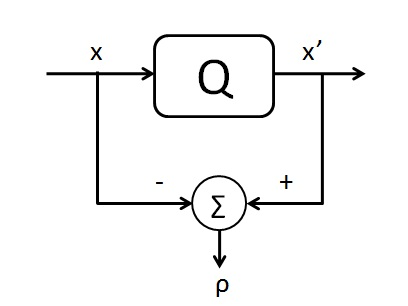
\includegraphics[scale=0.5]{Quantizer} 
\end{center}The set of possible values to the input of the quantizer maybe infinitely large but the output of the quantizer would always be either finite or countably infinite set of numbers. 
The x is the input signal to the quantizer and the x' is the output of the quantizer. The quantization noise is represented as $\rho$ which is the difference of the output and the input. This $\rho$ can be modeled in various ways which is explained in detail in later sections. The quantizer input output waveform looks like a staircase which suggests clearly that quantization is a nonlinear operation and hence modeling and analysis of quantization noise demands for separate and detailed analysis, which is precisely what will be looked into in this project. 
\subsection{Quantizing Theorem I and II} Widrow in \cite{Kollar} describes the statistical theory of Quantization where he explains how quantization noise in a digital control system or for that matter any other digital signal processing application could be modeled. Using assumptions of two theorems' validity, the quantization noise can be approximated as a PQN additive noise which is described in the next section. \\ 
The Quantizing Theorems I states that if the CF (Characteristic Function, $\phi$) of the Probability Density Function (PDF) of the the quantizer input x is band limited (which is obtained on taking Fourier transform (variable 'u') of the input signal PDF) such that:
\begin{equation}
\phi_x(u) = 0 ; |u| >\pi/q  
\end{equation}
then the CF of the input of the quantizer maybe derived uniquely from the CF of the output x', the same statement follows for PDF of the signals. In essence, the theorem states that the PDF's of input and output of the Quantizer are uniquely related to each other.
The Quantizing Theorem II on the other hand puts forward an important and a stronger result that the moment of the quantized variable (the output of quantizer) is equal to the moment of the sum of the input and a uniformly distributed noise which has a zero mean and mean square equal to $\frac{q^{2}}{12}$. 
\\The details of these theorem along with their proofs have been covered in detail in \cite{Widrow} the book on Quantization Noise.
\subsection{PQN Model: Additive Noise Approximation} To model the quantization noise in a form that is easy to analyze, we take help of the principle from statistics which states that, The PDF of the sum when two statistically independent signals are added together is equal to the convolution of the PDF's of the individual signals which implies that the CF of the sum would be just the product of the two individual CF's.
Hence, the PDF of Quantizer output x' $f_{x'}(x)$, which is a discrete signal equal to the samples of the smooth PDF of the the input signal added with a uniform noise n, $f_{x+n}(x)$. These two PDF's correspond to each other in such a way that the moments of the two are equal when quantizing theorems QT I and QT II are satisfied.   In this case, the quantizer can be replaced by Pseudo Quantization Noise (PQN), which is an additive uniform noise. This replacement by additive noise holds to a  very good approximation for Gaussian signals for $\sigma > q$ and even for higher values of q ($\sigma = q$). For other distributions, the approximation model is valid to a good approximation for low values of q.
\subsection{Noise Shaping Filter}
Noise Shaping is a technique used to modify the frequency spectra of the error signal in such a way that the noise power of the spectrum is more in the undesirable frequency band which leads to a higher SNR in the desirable frequency band. 
Considering analysis in the frequency domain, we have, on oversampling, according to the Nyquist Sampling Theorem the quantization noise is equal to $\frac{q}{\sqrt{12}}$ spread uniformly in the band of DC to $\frac{fs}{2}$.\cite{Interpolation}

where 

q=Value of an LSB
$f_{s}$=Sampling Rate

In sigma-delta ADC, oversampling technique is used to spread the quantization error noise over a bigger range of frequency, hence decreasing the noise power in the desired bandwidth. The SNR is further amplified by using a quantizer in the feedback loop which essentially shapes the noise power spectrum so that most of it lies outside the passband of the low pass filter which is designed to give the output as the desired frequency bandwidth only. \cite{SNR}
Similarly, a delta-sigma DAC \cite{Interpolation} uses a delta sigma modulator to shape the noise so that the effective quantization noise at lower frequencies is greatly reduced.

Consider for example the given system (see figure) where the input (denoted by x) which is in double precision, is fed into the quantizer. The quantizer rounds it off and feeds to the DAC according to the DAC's resolution, hence incurring quantization error. To achieve noise shaping the quantization error, denoted by e is fed back as shown. The output of the quantizer is denoted by x' and the following equations explain how noise shaping is beneficial.
\begin{center}
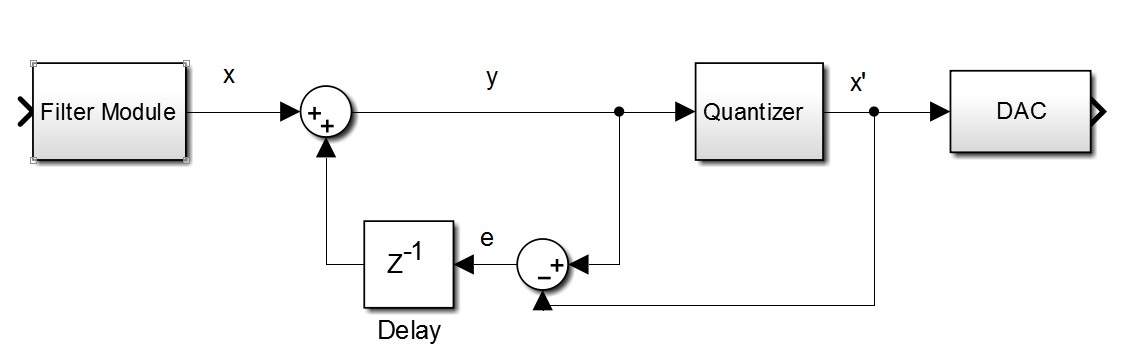
\includegraphics[scale=0.5]{NoiseShaping} 
\end{center}
From the block diagram (in time domain), we have,
\begin{equation}
y[n]=x[n]+e[n-1]
\end{equation}
\begin{equation}
e[n]=y[n]-x'[n]
\end{equation}
From equations (2) and (3) we have,
\begin{equation}
x'[n]=y[n]-e[n]
\end{equation}
Now taking the Z-Transform of equations (2) and (4), we have
\begin{equation}
Y(z)=X(z)+\frac{E(z)}{z}
\end{equation}
\begin{equation}
X'(z)=Y(z)-E(z)
\end{equation}
Now from equations (5) and (6), we get the final result which shows how quantization error is added to the input to form the output x', and since we have fed the error back we will see how the quantization noise is now shaped according to the transfer function we chose (in this case 1/z):
\begin{equation}
X'(z)=X(z)+E(z)(1-\frac{1}{z})
\end{equation}
The noise is shaped by a factor of $\frac{z-1}{z}$ which has a zero at z=1 and a pole at z=0. This means that at the frequency corresponding to z=0, the gain will be high and at frequency corresponding to z=1 the gain will be low since a zero is occurring there. In essence, we have a one-pole digital filter in front of us resulting due to the feedback of the error. In this way, noise shaping can be achieved to increase the SNR in the desired frequency band.
\section{Objectives}
\subsection{Software Tool}
Develop a software tool to design and analyze digital filters and controllers: The tool would be extensively used to design digital filters and test the performance and quantization noise effects on the control system. The simulation software would provide high precision calculations with almost zero quantization noise to obtain benchmark outputs (or so to say the desired specification for any kind of filter). The tool would be an improvement on the already existent tools related to this to accommodate the above and various other things such as analysis of sequential digital filters, checking of applicability of QT II model for the same which would enable us to know whether or not the replacement of nonlinear quantizer noise with additive  white PQN model holds or not for the given test case being simulated.
\subsection{Noise Shaping Filter for DAC}
The Digital to Analog Converter is among the main sources of quantization noise and hence this project aims to develop methods to mitigate the noise. Like in Delta-Sigma ADC’s the noise shaping filter helps to mitigate the quantization noise to a negligible level, a similar noise-shaping filter would be designed for the DAC in use so that the quantization noise effects could be minimized to a great extent. The DAC would be modeled in a simulator software and hence its performance and results of the noise shaping filter and possibly other methods to tackle the quantization noise would be studied using the simulation results from the software.  Also, in this project we would be studying various trade-offs in the design of DAC and digital compensator with respect to the design complexity, cost, performance, noise effects etc. . 
\subsection{Measurements and Calculations}
The project would involve measurements both virtually (i.e. on simulations) and on the real system. First, all the design strategies and ways to mitigate the quantization noise will be simulated using software tool(s) and then the measurements obtained from simulation would be compared to the measurements obtained in the real testing on the systems. Some integral quantities that shall be measured and used as performance indicator are quantization noise power spectrum, the SNR and the effects on SNR due to changes in various parameters. 
Mathematical calculations and derivations from theory of all the quantities being measured would also be performed in order to keep tabs with all results and to be assured of any inference made from the results and its conclusions. 
The transfer function of the digital filter would be designed using feedback control theory and also by applying proper optimization algorithms so as to achieve a compensator that works good from both points of view. The pole and zero placements of the transfer function would accordingly be done.  
\subsection{Assumptions}
The basic assumption which is valid for most cases as well, is that the Quantization noise is uncorrelated to the input signal wherever it occurs.
Moreover, All measurements and experiments will be under the assumption that QT II model is applicable, unless otherwise mentioned. This assumption enables us to replace the quantization noise source with white additive PQN source in the control loop. Also, for multiple quantizers in the same loop it shall be assumed that the two quantization noises are highly uncorrelated to each other and hence essentially white. 
We shall also assume that the signal is always scaled such that the quantizers are not underloaded or overloaded, thus assuming the absence of limit cycles and highly nonlinear behaviors. 

\section{Approach and Time-line}
Here are some milestones to look forward to throughout the project along with the expected time-line for each
\subsection{Software Tool and Quantization Noise Code} For the first week of the project, the focus would be mainly on familiarization with the software tool and with the quantization noise code existing. This would be done by testing the code at the 40 m Caltech Interferometer. The appropriate noise analysis and inferences would be carried out simultaneously.
\subsection{Quantization Noise Analysis of Digital aLIGO filters} After the initial testing and familiarization, it would be down to developing the software tool to enable it to perform an automated quantization noise analysis on various aLIGO filters. This part of the project is expected to be complete in around another two weeks, that would be Weeks 2-4 of the project time-line.
\subsection{Optimization of Filter Design}For the next two to three weeks, we would be optimizing the aLIGO filter designs against quantization noise using various design strategies and optimization methods. The analysis of the optimized filters would be done using the software tool.
\subsection{DAC Noise Shaping}The project would conclude with implementation of noise shaping in the DACs. The current LIGO digital control systems involve the DACs which do not take advantage of noise shaping. If the noise shaping is implemented successfully in the DACs, then the quantization noise could be reduced to a great extent in the desired frequency band. This part of the project could take upto three weeks.

\begin{thebibliography}{13}  
\bibitem{LIGO} B. P. Abott et. al.,  
				\emph{LIGO: the laser Interferometer Gravitational Wave Observatory} 							\url{http://dx.doi.org/10.1088/0034-4885/72/7/076901}
\bibitem{GWD} \emph{On Gravitational Wave Detection: }
			\url{https://nodus.ligo.caltech.edu:30889/wiki/doku.php?id=gw_detection_101_for_surf}

\bibitem{Interferometer} Frederick J Raab, \emph{Overview of LIGO Instrumentation}
\bibitem{WhyDigital} \emph{Why Digital Control instead of Analogue?} 												\url{http://www.uotechnology.edu.iq}

\bibitem{Control} L. Carbone et al., \emph{Sensors and Actuators for the Advanced LIGO Mirror Suspensions}
									\url{http://arxiv.org/pdf/1205.5643v1/}
									
\bibitem{Widrow} Widrow and Kollar, \emph{Quantization Noise} 				\url{http://www.mit.bme.hu/books/quantization}

\bibitem{Dehner} Dehner, \emph{Noise Optimized Filter Design} 		\url{https://dx.doi.org/10.1016/s0165-1684(03)00075-6}

\bibitem{AnalogDevices} \emph{Application Note on Sigma Delta ADC's and DAC's:} \url{http://www.analog.com/media/en/technical-documentation/application-notes/292524291525717245054923680458171AN283.pdf}

\bibitem{Interpolation}\emph{Oversampling Interpolating DAC}	\url{http://www.analog.com/media/cn/training-seminars/tutorials/MT-017.pdf}

\bibitem{SNR} \emph{Signal to Noise Ratio} 
				\url{http://www.analog.com/media/en/training-seminars/tutorials/MT-001.pdf}
				
\bibitem{Sheingold} D. H. Sheingold, \emph{Analog-Digital Conversion Handbook}
\bibitem{Tretter} S. A. Tretter, \emph{Introduction to Discrete Time Signal Processing John Wiley and Sons, New York, 1976}
\bibitem{Kollar} B. Widrow and I. Kollar, \emph{Statistical Theory of Quantization}

\end{thebibliography}        
\end{document} % The document ends here
